In questo capitolo è descritto il processo di creazione del dataset usato per valutare il sistema di correzione sviluppato.\\
Nella \autoref{dst:intro} sono discussi gli obiettivi e le caratteristiche che il dataset deve avere. Nella \autoref{dst:creazione} sono delineate la metodologia di creazione e la struttura del dataset. Nella \autoref{dst:perturbazione} è descritto il processo introduzione di errori all'interno delle frasi per simularne l'acquisizione tramite OCR, detto perturbazione. Nella \autoref{dst:configurazione} infine, sono discussi i parametri e la configurazione del dataset.
\section{Introduzione}
\label{dst:intro}
Lo sviluppo di un sistema di OCR post-processing non può prescindere dall'esecuzione di test per valutare, migliorare e confrontare le soluzioni adottate. Ciò rende necessario l'utilizzo di un dataset sul quale poter eseguire tutte le batterie di test necessarie. Tale dataset deve inoltre essere strutturato in modo tale da permettere di calcolare facilmente le metriche descritte nella \autoref{sec:test_metriche}. Se infatti lo scopo di un sistema di OCR post-processing è quello di correggere gli errori introdotti dai software di OCR, è necessario conoscere la posizione degli errori per controllare se siano stati corretti o meno.\\
La soluzione più semplice a questo problema è quella di disporre, per ogni frammento del dataset, sia del testo acquisito tramite OCR (e quindi contenente errori), sia del testo originale, detto anche ground truth. Non è però semplice trovare dataset di questo tipo, specialmente se in lingua italiana. Spesso, infatti, è necessario che la ground truth sia acquisita manualmente con un grosso dispendio di tempo e risorse: a causa di ciò, questo approccio non è stato considerato percorribile ai fini della tesi.\\
Si è invece deciso di adottare un approccio differente, che consiste nell'introduzione artificiale di errori all'interno di testo nativamente digitale (e quindi senza errori) per simularne l'acquisizione tramite OCR. I vantaggi del processo appena descritto, detto "perturbazione", sono riassumibili nei seguenti punti:
\begin{itemize}
 \item Produrre il dataset, una volta definita la funzione che esegue la perturbazione, è molto meno oneroso in termini di tempo e risorse. L'unico requisito è quello di procurarsi una collezione sufficientemente ampia di testo in formato digitale. Ciò è relativamente semplice, e può essere fatto, ad esempio, tramite web scraping. 
 \item \E\ possibile definire arbitrariamente l'intensità e la tipologia degli errori nel testo tramite l'uso di diverse funzioni di perturbazione. Ciò permette, dato un singolo testo di partenza, di ottenere testi con diverse intensità e tipologie di errori. In questo modo si rende possibile valutare le performance del sistema di OCR post-processing al variare delle condizioni del testo dato in input.
\end{itemize}
Il principale rischio che si corre utilizzando l'approccio appena descritto risiede nel fatto che il testo perturbato potrebbe non rispecchiare fedelmente gli errori presenti in testo acquisito realmente tramite software di OCR.

\vfill
\section{Creazione del dataset}
\label{dst:creazione}
Il dataset di partenza è una collezione di 15073 documenti in formato JSON, ottenuti mediante il web scraping del sito ufficiale del vaticano \url{www.vatican.va}. I documenti contengono preghiere, lettere, discorsi, encicliche ecc. editi da figure ecclesiastiche dal 1439 al 2021.\\
Ogni documento è caratterizzato dalla struttura descritta in \autoref{tab:dst_docstrut}.


\begin{table}[H]
\centering
\begin{tabular}{ll}
\textbf{Nome campo} & \textbf{Contenuto} \\ \hline
title & Titolo del documento \\
description & Insieme di keyword del documento\\
author & Autore del testo nel documento \\
creator & Coincide con author \\
language & Codice della lingua del documento (es. it, fr) \\
date & Data di redazione del documento \\
url & Url da cui è stato il documento \\
class & Tipologia di documento (es. discorso, preghiera...)\\
text & Testo completo estratto dal documento (titolo compreso)\\
url\_references & Link al feed RSS del sito del vaticano \\
text\_references & Posizione della pagina nella gerarchia del sito\\
italic & Testo estratto in corsivo nella pagina \\
paragraphs & Testo estratto diviso in paragrafi contenenti id e testo
\end{tabular}
\caption{Struttura di un documento nel dataset}
\label{tab:dst_docstrut}
\end{table}

Dato il dataset descritto, l'obiettivo è quello di trasformalo in un formato consono al testing. Nello specifico, è necessario frammentare il testo contenuto nei documenti in frasi di lunghezza minima e massima predeterminate. Le ragioni di questa decisione sono approfondite nel \autoref{sec:test}, ma, in breve, spezzare il testo in frammenti più piccoli facilita il processo di allineamento delle frasi e quindi la valutazione delle correzioni. Per ognuno dei frammenti si vogliono poi produrre più versioni perturbate con diverse funzioni di perturbazione. Infine, è necessario che le frasi siano accompagnate da dei metadati che consentano la ricomposizione del testo originale mediante il riordinamento dei frammenti.\\
La creazione del dataset per il testing, descritta nelle prossime sezioni, segue dunque le seguenti fasi:
\begin{enumerate}
\item Filtraggio lingue
\item Estrazione
\item Frammentazione
\item Filtraggio paragrafi
\item Perturbazione
\item Riduzione
\end{enumerate}

\paragraph{Filtraggio lingue}
In questa fase vengono filtrati tutti i documenti non presenti fra lingue scelte. Dato l'insieme dei documenti $D$ e l'insieme delle lingue consentite $L$, l'insieme filtrato dei documenti $D_{fl}$ si ottiene come segue:
\begin{equation}
D_{fl} = \{d\ \forall d \in D\ |\ \textit{language}_d \in L  \} 
\end{equation}
dove, dato un documento $d \in D$, $\textit{language}_d$ è la lingua in cui è redatto. Le lingue scelte per la creazione del dataset sono elencate nella \autoref{dst:configurazione}.

\paragraph{Estrazione}
In questa fase sono scartati i campi superflui ai fini del testing, e sono mantenuti solo i paragrafi assieme ad alcuni metadati utili a ricomporre il testo originale in seguito. \E\ possibile formalizzare la prima parte di questa fase come segue:
\begin{equation}
D_{es1} = \{ meta({paragraphs}_d)\ \forall d \in D  \}
\end{equation}
dove la funzione $meta$ aggiunge ai paragrafi in ${paragraphs}_d$ l'id del documento di provenienza. Si ottiene quindi un insieme di insiemi di paragrafi, dove ogni paragrafo è strutturato come in \autoref{tab:dst_parstrut}.

\begin{table}[H]
\centering
\begin{tabular}{ll}
\textbf{Nome campo} & \textbf{Contenuto} \\ \hline
text  & Testo contenuto nel paragrafo\\
parId & Codice del paragrafo all'interno del documento \\
docId & Codice del documento di provenienza del paragrafo.
\end{tabular}
\caption{Struttura di un paragrafo}
\label{tab:dst_parstrut}
\end{table}

La fase di estrazione è completata appiattendo le liste di paragrafi nell'insieme $D_{es1}$ 
\begin{equation}
D_{es} = \bigcup\limits_{p \in D_{es1}} p
\end{equation}
$D_{es}$ contiene quindi tutti i paragrafi del dataset iniziale strutturati come mostrato in \autoref{tab:dst_parstrut}.



\paragraph{Frammentazione}
Lo scopo di questa fase è quello di scomporre i paragrafi estratti nella fase precedente in frammenti più brevi, detti frasi, con le seguenti caratteristiche:
\newcommand{\lmin}{$l_{min}$}
\newcommand{\lmax}{$l_{max}$}
\begin{itemize}
\item Ogni frase è disgiunta dalle altre frasi estratte dal medesimo paragrafo.
\item Ogni frase è compresa fra una lunghezza minima \lmin\ e una lunghezza massima \lmax\ (\autoref{dst:configurazione}).
\end{itemize}

Dato quindi il testo di un paragrafo $text_p$, la frammentazione avviene secondo la seguente procedura:

\begin{enumerate}
\item Se la lunghezza di $text_p$ è minore di \lmin, non si procede e si scarta la stringa.
\item Si divide $text_p$ su un segno di punteggiatura fra i seguenti: "?", "!", ";", ":", ".", ",". Se sono disponibili più opzioni (ovvero più punti in cui è possibile dividere su segni di punteggiatura) si divide nel punto minore o uguale a \lmax\ che più si avvicina al valore di \lmax. La parte a sinistra del punto di divisione è una frase estratta. La parte a destra invece viene riutilizza come input della procedura di frammentazione, tornando al punto 1. Se non fosse possibile eseguire alcuna divisione, si passa al punto successivo.
\item Si divide $text_p$ su uno spazio. Se sono disponibili più opzioni (ovvero più punti in cui è possibile dividere su uno spazio) si divide nel punto minore o uguale a \lmax\ che più si avvicina al valore di \lmax. La parte a sinistra del punto di divisione è una frase estratta. La parte a destra invece viene riutilizza come input della procedura di frammentazione, tornando al punto 1. Se non fosse possibile eseguire alcuna divisione, si passa al punto successivo.
\item Se la lunghezza di $text_p$ è minore di \lmax, $text_p$ è aggiunto alle frasi estratte. Altrimenti, si divide $text_p$ in posizione \lmax. La parte a sinistra del punto di divisione è una frase estratta. La parte a destra invece viene riutilizza come input della procedura di frammentazione, tornando al punto 1. 
\end{enumerate}

La procedura appena descritta fa in modo che i frammenti approssimino il più possibile \lmax, evitando il più possibile introdurre errori. Spezzare un paragrafo nel mezzo di una parola, ad esempio, andrebbe a creare due frammenti contenenti degli errori (uno sulla parola finale del primo, l'altro sulla parola iniziale del secondo.\\
Durante la frammentazione ogni frammento ritiene i metadati relativi al documento e al paragrafo di appartenenza. In più, si aggiunge un ulteriore campo per tenere traccia della posizione del frammento all'interno del paragrafo di appartenenza. In questo modo, è possibile ricomporre un documento in secondo momento. Ogni frase prodotta rispetta il seguente schema:
\begin{table}[H]
\centering
\begin{tabular}{ll}
\textbf{Nome campo} & \textbf{Contenuto} \\ \hline
text  & Testo contenuto nella frase\\
parId & Codice del paragrafo di provenienza \\
docId & Codice del documento di provenienza.\\
parPos & Posizione della frase all'interno del paragrafo di provenienza\\
\end{tabular}
\caption{Struttura di una frase}
\label{tab:dst_frasestrut}
\end{table}

La frase di frammentazione si può quindi formalizzare in due step. Nel primo step, ogni paragrafo viene frammentato nella lista delle sue frasi:
\begin{equation}
D_{fr1} = \{ extr(p)\ \forall p \in D_{es}  \}
\end{equation}
dove $extr$ è la funzione che estrae le frasi secondo la procedura descritta precedentemente, producendo un insieme di frasi strutturate come mostrato in \autoref{tab:dst_frasestrut}. Nel secondo step si appiattisce l'insieme di insiemi che si è andato a creare, per ottenere insieme di frasi:
\begin{equation}
D_{fr} = \bigcup\limits_{f \in D_{fr1}} f
\end{equation}

\paragraph{Filtraggio paragrafi}
Lo scopo di questa fase è quello di rimuovere dal dataset tutti le frasi che appartengono al primo o all'ultimo paragrafo di un documento. Ciò si rende necessario perchè questi paragrafi spesso contengono intestazioni o piè di pagina ripetitivi andrebbero a sporcare il dataset. Ad esempio, l'ultimo paragrafo contiene spesso una frase simile  a \textit{"© Copyright 2004 - Libreria Editrice Vaticana"}, mentre il primo spesso contiene solamente una data.\\
\E\ definita la seguente funzione $\textit{maxPar}$ che, data una frase $f \in D_{fr}$, indica se $f$ appartiene all'ultimo paragrafo del documento da cui è stata estratta:
\begin{equation}
  maxPar(f) =
    \begin{cases}
      1 & \text{se $f$ appartiene all'ultimo paragrafo di $docId_f$}\\
      0 & \text{altrimenti}
    \end{cases}       
\end{equation}
L'operazione di filtraggio dei paragrafi può quindi essere formalizzata come segue:
\begin{equation}
D_{fp} = \{ f \ \forall f \in D_{fr}\ |\  parId_{f} \neq 0 \wedge maxPar(f) = 0     \}
\end{equation}

\paragraph{Perturbazione}
Durante la fase di perturbazione, per ogni frase del dataset sono generate le sue versioni perturbate. Ogni versione perturbata di una frase viene generata da una diversa funzione di perturbazione applicata alla frase stessa. Il funzionamento delle funzioni di perturbazione è spiegato nella \autoref{dst:perturbazione}, mentre le esatte funzioni per la creazione del dataset sono elencate nella \autoref{dst:configurazione}.\\
Viene chiamata $F_p$ la lista $[p_1,...,p_n]$ delle funzioni di perturbazione utilizzate, in cui ogni $p_i$ è identificata da un codice. Data una stringa di testo $s$, la sua versione perturbata dalla funzione $p_i$ corrisponde a $p_i(s)$.\\
Data quindi una frase $f \in D_{fr}$ strutturata come in \autoref{tab:dst_frasestrut}, e lista delle funzioni di perturbazione $F_p$, si definisce come $P_{list}$ l'insieme delle frasi perturbate $[p_1(text_f),...,p_n(text_f)]$ la cui rappresentazione è schematizzata in \autoref{tab:dst_frasepert}.

\begin{table}[H]
\centering
\begin{tabular}{ll}
\textbf{Codice funzione perturbazione} & \textbf{Frase perturbata} \\ \hline
$nome\_func_1$ & $ p_1(f)$\\
$nome\_func_2$ & $ p_2(f)$\\
... &  ...\\
$nome\_func_n$ & $ p_n(f)$\\
\end{tabular}
\caption{Struttura delle frasi perturbate}
\label{tab:dst_frasepert}
\end{table}

Si definisce inoltre la funzione $applyPert$ che, data una frase $f \in D_{fr}$, produce un sample aggiungendo a $f$ un campo con le sue versioni perturbate della frase originale. Un sample è strutturato come in \autoref{tab:dst_samplestrut}.

\begin{table}[H]
\centering
\begin{tabular}{ll}
\textbf{Nome campo} & \textbf{Contenuto} \\ \hline
text  & Testo contenuto nella frase non perturbata\\
parId & Codice del paragrafo di provenienza \\
docId & Codice del documento di provenienza.\\
parPos & Posizione della frase all'interno del paragrafo di provenienza\\
perturbed & Frasi perturbate ($[p_1(text_f),...,p_n(text_f)]$)
\end{tabular}
\caption{Struttura di una frase}
\label{tab:dst_samplestrut}
\end{table}


La fase di perturbazione può quindi essere formalizzata come segue:
\begin{equation}
D_{pe} = \{applyPert(f)\ \forall f \in D_{fp}\}
\end{equation}

\paragraph{Riduzione}
Lo scopo della fase di riduzione è quello di creare una versione ridotta del dataset, ovvero di ridurne il numero di elementi. Ciò è reso necessario dal fatto che il testing può essere significativamente oneroso in termini di tempo e risorse, specialmente su dataset troppo ampi.\\
Data quindi la dimensione del dataset ridotto $n$ (i cui valori sono specificati nella \autoref{dst:configurazione}), il dataset $D_{re}$ è un sottoinsieme di $n$ elementi estratti casualmente da $D_{pe}$:
\begin{equation}
D_{re} \subset D_{pe} \wedge |D_{re}| = n
\end{equation}
Dopo aver eseguito la fase di riduzione, la costruzione del dataset può dirsi completata.


\section{Perturbazione}
\label{dst:perturbazione}
Data una stringa $s$, lo scopo del processo di perturbazione è quello produrre una stringa $s\prime$ nella quale sono introdotti degli errori per simulare l'acquisizione del testo tramite OCR. Per permettere l'introduzione controllata e a diverse intensità degli errori è stato sviluppato un sistema modulare e componibile, che sarà illustrato in questa sezione.

\subsection{Moduli di perturbazione}
\label{dst:modpert}
La componente base del sistema di perturbazione è il modulo di perturbazione. Un modulo di perturbazione non è altro che una funzione che modella l'inserimento di una specifica tipologia di errore. Ciò significa che per ogni tipologia di errore modellata si rende necessaria la creazione di un modulo di perturbazione. Ad esempio, è possibile definire un modulo di perturbazione che modelli la sostituzione di alcuni caratteri, o un modulo che inserisca della punteggiatura spuria. \\
Tutti i moduli di perturbazione, data una lista ordinata di token, introducono errori mediante la modifica, la divisione, l'unione o la cancellazione di uno o più token. \\
Data una lista di token $list_t = [t_1,...,t_n]$,
Il funzionamento di un modulo di perturbazione si può dividere nelle seguenti tre fasi:

\begin{enumerate}
	\item \textbf{Raggruppamento}: I token sono raggruppati in gruppi consecutivi e disgiunti di $k$ elementi, dove $k$ varia a seconda della tipologia di modulo di perturbazione. \\
La fase di raggruppamento è quindi definita come segue:
\begin{equation}
group: [t_1,...,t_n] \rightarrow [g_1,...,g_q]
\end{equation}
dove ogni $g_i$ è un gruppo di token $[t_1,..., t_k  ]$ e $q = \lceil n/k \rceil$.\\
	
Ad esempio, data la lista di token \textit{['Nel', 'mezzo', 'del', 'cammin', 'di', 'nostra', 'vita']} e $k = 2$, i token sono raggruppati nel seguente modo: \textit{['Nel', 'mezzo'], ['del', 'cammin'], ['di', 'nostra'], ['vita']}.
	
	\item \textbf{Perturbazione}: Ogni tipologia di modulo di perturbazione è caratterizzata da una specifica funzione di perturbazione $f_{pert}$
\begin{equation}
f_{pert}: [t_1,..., t_k  ] \rightarrow [t'_1,..., t'_j]
\end{equation}
che introduce errori mediante la modifica, la divisione, l'unione o la cancellazione dei token in un determinato gruppo, con una probabilità $p$ definita per ogni modulo. Un qualsiasi gruppo di token $g \in [g_1,...,g_q]$ viene perturbato o meno secondo la seguente funzione:
\begin{equation}
f_{map}(g) =
    \begin{cases}
      f_{pert}(g) & \text{con probabilità $p$}\\
      g & \text{con probabilità $1-p$}
    \end{cases}  
\end{equation}
\E\ quindi possibile definire la fase di perturbazione come:
\begin{equation}
pert: [g_1,...,g_q] \rightarrow [g\prime_1,...,g\prime_q]
\end{equation}
dove $g\prime_i = f_{map}(g_i)\ \forall i \in [1..q]$.


Ad esempio, si supponga di avere un modulo in cui $f_{pert}$ sia definita come:
\begin{equation}
f_{ex}([t_1,t_2]) = [t_1 \frown t_2]
\end{equation}
La funzione appena definita concatena i due token all'interno di gruppo, restituendo un gruppo formato da un solo token. Si consideri l'esempio nel punto precedente, e si supponga che l'unico gruppo affetto da perturbazione sia il secondo. Si ha quindi che $f_{pert}(\textit{['del', 'cammin']}) = \textit{['delcammin']}$, e quindi alla fine di questa fase si ottiene: \textit{['Nel', 'mezzo'], ['delcammin'], ['di', 'nostra'], ['vita']}.

\item \textbf{Appiattimento}: la fase di appiattimento è l'opposto di quanto avviene durante il raggruppamento. I gruppi di token sono raggruppati nuovamente in un'unica lista:
\begin{equation}
flat: [g\prime1,...,g\prime_q] \rightarrow [t_1,...,t_m]
\end{equation}
dove $m$ potrebbe coincidere o meno con $n$ a seconda del tipo di perturbazione avvenuta.\\
Riprendendo l'esempio precedente, il risultato di questa fase è: \textit{['Nel', 'mezzo', 'delcammin', 'di', 'nostra', 'vita']}
\end{enumerate}

Come si può notare, un modulo riceve in input una lista di token e fornisce in output un'altra lista di token. Ciò rende possibile concatenare più moduli, per introdurre più di un tipo di errore all'interno di una sequenza di token. Questa eventualità è descritta nella \autoref{sec:dst:pipeline} e nella \autoref{sec:dst:superpipeline}.\\
Quanto descritto finora non basta a soddisfare lo scopo della perturbazione, che è quello di trasformare una stringa in una nuova stringa contenente degli errori. Tale funzione è resa possibile dai moduli speciali, che sono approfonditi nella \autoref{sec:dst_modspec}.\\
Dal funzionamento dei moduli di perturbazione si evince come la funzione $f_{pert}$ caratterizzi il modulo modellando il tipo di errore che esso va ad introdurre. Sono quindi stati creati i seguenti moduli, ognuno dei quali è caratterizzato da una diversa funzione di perturbazione:

\newcommand{\mss}{$M_{ss}$}
\newcommand{\mps}{$M_{ps}$}
\newcommand{\mpi}{$M_{pi}$}
\newcommand{\mhm}{$M_{hm}$}
\newcommand{\mcr}{$M_{cr}$}

\begin{itemize}
\item Modulo di space splitting (\mss)
\item Modulo di punctuation splitting (\mps)
\item Modulo di punctuation insertion (\mpi)
\item Modulo di hyphen merging (\mhm)
\item Modulo di characters replacement (\mcr)
\end{itemize}

Ognuno di questi moduli è stato creato per modellare un particolare tipo di errore. Le tipologie di errore modellate sono state decise in base all'analisi di documenti il cui testo è stato acquisito tramite OCR. Più nello specifico, si tratta delle trascrizioni dei dibattiti parlamentari della prima e della seconda legislatura della repubblica italiana.

\subsubsection{Modulo di space splitting}
Il modulo di space splitting modella l'errore in cui le lettere di una parola sono intramezzate da degli spazi. Siccome la perturbazione avviene su un singolo token, i token in input sono raggruppati in gruppi di un token ($k = 1$). Si definisce dunque la funzione di perturbazione del modulo:
\begin{equation}
f_{pert\_split}([t_1]) = [f_{split}(t_1)]
\end{equation}
in cui $f_{split}$ è la funzione che aggiunge uno spazio dopo ogni carattere di un token.
\paragraph{Esempi}
\begin{equation}
f_{pert\_split}(["cammin"]) = ["c\ a\ m\ m\ i\ n\ "]
\end{equation}
\begin{equation}
f_{pert\_split}(["nostra"]) = ["n\ o\ s\ t\ r\ a\ "]
\end{equation}

\subsubsection{Modulo di punctuation splitting}
Il modulo di punctuation splitting modella l'errore in cui una o più occorrenze di un segno di punteggiatura intramezzano i caratteri di una parola.
Siccome la perturbazione avviene su un singolo token, i token in input sono raggruppati in gruppi di un token ($k = 1$). Si definisce dunque la funzione di perturbazione del modulo:
\begin{equation}
f_{pert\_punctsplit}([t_1]) = [f_{punctsplit}(t_1,punct)]
\end{equation}
Assumendo che:
\begin{itemize}
\item $punct$ sia il segno di punteggiatura che è intramezzato agli spazi,
\item un token $t$ sia una sequenza di caratteri $[c_1,...,c_n]$, ovvero $|t| = n$,
\item sia definito un numero casuale $x \in \mathbb{N}\ |\ 1 \leq x \leq n$
\end{itemize}
è possibile definire $f_{punctsplit}$ come:
\begin{equation}
f_{punctsplit}(t,punct) = 
\begin{cases}
	[c1,...,c_x] \frown\ punct \frown f_{punctsplit}([c_{x+1},...,c_n],punct)&\text{se $x < |t|$}\\
	t	&\text{se $x \geqslant |t|$}
\end{cases}
\end{equation}
Informalmente, la funzione aggiunge un carattere $punct$ ogni $x$ caratteri all'interno di $t$.

\paragraph{Esempi}
\begin{equation}
f_{punctsplit}(\textit{"cammin"},\textit{","}) = \textit{"ca,mm,in"}\ (x = 2)
\end{equation}
\begin{equation}
f_{punctsplit}(\textit{"mezzo"},\textit{","}) = \textit{"m,e,z,z,o"}\ (x = 1)
\end{equation}


\subsubsection{Modulo di punctuation insertion}
Il modulo di punctuation insertion modella l'errore in cui un segno di punteggiatura è aggiunto fra due token, senza quindi dividere in due un singolo token.
Siccome la perturbazione avviene su un singolo token, i token in input sono raggruppati in gruppi di un token ($k = 1$). Si definisce dunque la funzione di perturbazione del modulo:
\begin{equation}
f_{pert\_insertion}([t_1]) = [t_1, punct]
\end{equation}
dove $punct$ è il segno di punteggiatura da aggiungere.
\paragraph{Esempi} Data la sequenza di gruppi di token \textit{\underline{['Nel']}, ['mezzo'], ['del'], \underline{['cammin']}, ['di'], ['nostra'], ['vita']}, dove i gruppi sottolineati sono quelli da perturbare, e dato $punct = "."$, si ha che:
\begin{equation}
f_{pert\_insertion}(\textit{["Nel"]},\textit{"."}) = \textit{["Nel","."]}\ 
\end{equation}
\begin{equation}
f_{pert\_insertion}(\textit{["cammin"]},\textit{"."}) = \textit{["cammin","."]}\ 
\end{equation}
Quindi, applicata la fase di appiattimento, la sequenza finale risulta: \textit{['Nel'], ['.'], ['mezzo'], ['del'], ['cammin'], ['.'], ['di'], ['nostra'], ['vita']}.

\subsubsection{Modulo di hyphen merging}
Il modulo di hypen merging modella l'errore in cui due parole consecutive vengono unite da un trattino. Dovendo unire due token tra di loro, la perturbazione avviene in gruppi di due token, quindi si ha $k = 2$. Si definisce dunque la funzione di perturbazione del modulo:
\begin{equation}
f_{hyphen}([t_1,t_2]) = [t_1\frown \textit{"-"} \frown t_2]
\end{equation}

\paragraph{Esempio} Data la sequenza di gruppi di 2 token \textit{['Nel', 'mezzo'], ['del', 'cammin'], \underline{['di', 'nostra']}, ['vita']}, dove il gruppo sottolineati sono quello da perturbare, si ha che:
\begin{equation}
f_{hyphen}(\textit{["di", "nostra"]}) = \textit{["di-nostra"]}
\end{equation}
Quindi, applicata la fase di appiattimento, la sequenza finale risulta: \textit{['Nel', 'mezzo'], ['del', 'cammin'], {['di-nostra']}, ['vita']}.

\subsubsection{Modulo di characters replacement}
Il modulo di characters replacement modella l'errore in un cui avviene la cancellazione, l'aggiunta o la sostituzione di uno o più caratteri all'interno di un token. Siccome la perturbazione avviene su un singolo token, i token in input sono raggruppati in gruppi di un token ($k = 1$). Si definisce dunque la funzione di perturbazione del modulo:
\begin{equation}
f_{charrepl}([t_1]) = [f_{alternative}(t_1)]
\end{equation}
Per ogni token $t$ che viene perturbato, esiste un insieme di 5 versioni errate di $t$, detto $A_t = [a_{t1},...,a_{t5}]$, generato sulla base di una distribuzione di errori preesistente. La funzione $f_{alternative}$ rimpiazza $t$ con una delle alternative in $A_t$:
\begin{equation}
f_{alternative}(t) = a_{ti}
\end{equation}
dove $a_{ti} \in A_t$ e $i$ è un numero intero casuale fra 1 e 5.

\paragraph{Esempio} Sia dato il token \textit{"cammin"} e si supponga l'insieme delle versioni errate del token essere $A_{cammin} = [\textit{'cmmin', 'camniin', 'cdmmn', 'camin', 'cammiii'}]$. Si sceglie quindi in modo casuale un token dall'insieme $A_{cammin}$:
\begin{equation}
f_{alternative}(\textit{"cammin"}) = a_{cammin\_2} ="camniin"
\end{equation}


\subsection{Moduli speciali}
\label{sec:dst_modspec}
Come si è visto nella sottosezione precedente, i moduli di perturbazione lavorano su sequenze di token, nelle quali introducono degli errori. \E\ però necessario, come accennato all'inizio della \autoref{dst:perturbazione}, che la perturbazione prenda in input e restituisca come output delle stringhe. Sono quindi definiti due moduli, detti moduli speciali, che hanno lo scopo di convertire una stringa in una sequenza di token e viceversa:
\newcommand{\mto}{$M_{to}$}
\newcommand{\mde}{$M_{de}$}
\begin{itemize}
\item Modulo di tokenizzazione (\mto)
\item Modulo di detokenizzazione (\mde)
\end{itemize}

\subsubsection{Modulo di tokenizzazione}
Il modulo di tokenizzazione ha lo scopo di tokenizzare una qualsiasi stringa $s \in S$ in una lista $[t_1,...,t_n]$ di token:
\begin{equation}
tok: S \rightarrow [t_1,...,t_n]
\end{equation}
\paragraph{Esempio}
Data la frase $s_{ex} = \textit{"Nel mezzo del cammin di nostra vita"}$  
\begin{equation}
tok(s_{ex}) = \textit{['Nel', 'mezzo', 'del', 'cammin', 'di', 'nostra', 'vita']}
\end{equation}

\subsubsection{Modulo di detokenizzazione}
Il modulo di tokenizzazione ha lo scopo di detokenizzare, ovvero di eseguire il processo contrario alla tokenizzazione, una lista di token $[t_1,...,t_n]$ in una stringa $s \in S$.
\begin{equation}
detok: [t_1,...,t_n] \rightarrow S
\end{equation}
\paragraph{Esempio}
Data la sequenza di token $T_{ex} =$ \textit{['Nel', 'mezzo', 'del', 'cammin', 'di', 'nostra', 'vita']}.
\begin{equation}
detok(T_{ex}) = \textit{"Nel mezzo del cammin di nostra vita"}
\end{equation}



\subsection{Pipeline}
\label{sec:dst:pipeline}
Come accennato nelle sottosezioni precedenti, ogni modulo di perturbazione modella un diverso tipo di errore. In realtà, in un testo estratto tramite OCR sono presenti più tipologie di errori. \E\ quindi necessario utilizzare più moduli di perturbazione in sequenza per ottenere una perturbazione verosimile. Considerando che ogni modulo di perturbazione è considerabile come una funzione con dominio e codominio coincidenti $T$ (ogni elemento del dominio e codominio $T$ è una lista di token $[t_1,...,t_n]$ con $ n \in \mathbb{N} \wedge n \geqslant 0$), è possibile concatenare più moduli insieme tramite composizione:
\begin{equation}
m_k \circ m_{k-1} \circ m_{k-2} \circ ... \circ m_1
\end{equation}
dove ogni $m_i$ è istanza di un modulo di perturbazione. La funzione composta non può però trattare stringe, ma solo sequenze di token. Ciò è ovviabile attraverso l'aggiunta dei moduli speciali di tokenizzazione e detokenizzazione all'inizio e alla fine della composizione. La funzione risultante prende il nome di pipeline:
\begin{equation}
Pipeline: detok \circ m_k \circ m_{k-1} \circ m_{k-2} \circ ... \circ m_1 \circ tok
\end{equation}
Data quindi una stringa $s \in S$, la stringa perturbata $s\prime \in S$ è ottenuta come:
\begin{equation}
Pipeline(s) = s\prime
\end{equation}

\paragraph{Esempio}
Si definisca una pipeline $p_{ex}$ composta come indicato in \autoref{tab:dst_pex}.

\begin{table}[H]
\centering
\begin{tabular}{ccccc}
\textbf{Posizione} & \textbf{Nome istanza} & \textbf{Tipo Modulo} & \textbf{p} & \textbf{punct}\\ \hline
1	& $m_{to}$	& \mto	& n.d 	& n.d 	\\
2	& $m_{cr}$	& \mcr	& 0.3	& n.d 	\\
3	& $m_{ss}$	& \mss	& 0.1	& n.d 	\\
4	& $m_{pi}$	& \mpi	& 0.1	& , 	\\
5	& $m_{de}$	& \mde	& n.d 	& n.d 	\\
\end{tabular}
\caption{Struttura della pipeline $p_{ex}$}
\label{tab:dst_pex}
\end{table}

$p_{ex}$ corrisponde dunque alla seguente funzione, schematizzata anche in \autoref{fig:dst_pex}.
\begin{equation}
p_{ex} = m_{de} \circ m_{pi} \circ m_{ss} \circ m_{cr} \circ m_{to}
\end{equation}

\begin{figure}[H]
\centering
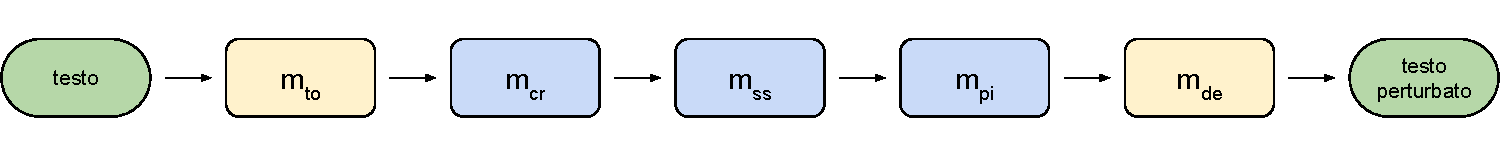
\includegraphics[width=\textwidth]{immagini/dataset/pex}
\caption{Schema della pipeline $p_{ex}$}
\label{fig:dst_pex}
\end{figure}

Data una stringa di esempio $s_{ex} = $ \textit{"Nel mezzo del cammin di nostra vita"}, è mostrata in seguito la sequenza dei passaggi che portano alla perturbazione della frase:
\begin{enumerate}
\setcounter{enumi}{-1}
\item ($s_{ex}$)\\
\textit{"Nel mezzo del cammin di nostra vita"}

\item $m_{to}(s_{ex})$\\
\textit{['Nel', 'mezzo', 'del', 'cammin', 'di', 'nostra', 'vita']}

\item $m_{cr}(m_{to}(s_{ex}))$\\
\textit{['Nel', \underline{'inezzo'}, 'del', \underline{'camniin'}, 'di', 'nostra', 'vita']}

\item $m_{ss}(m_{cr}(m_{to}(s_{ex})))$\\
\textit{['Nel', 'inezzo', 'del', \underline{'c a m n i i n'}, 'di', 'nostra', 'vita']}

\item $m_{pi}(m_{ss}(m_{cr}(m_{to}(s_{ex}))))$\\
\textit{['Nel', 'inezzo', 'del', 'c a m n i i n', 'di', \underline{','} , 'nostra', 'vita']}

\item $m_{de}(m_{pi}(m_{ss}(m_{cr}(m_{to}(s_{ex})))))$\\
\textit{"Nel inezzo del c a m n i i n di, nostra vita"}
\end{enumerate} 

Si sottolinea come questa sia solo una delle possibili perturbazioni di $s_{ex}$: essendoci nella perturbazione una componente aleatoria, ogni esecuzione di una pipeline su uno stesso input può dare risultati diversi.


\subsection{Superpipeline}
\label{sec:dst:superpipeline}
Una pipeline di perturbazione perturba il testo in modo uniforme: ogni frase perturbata con una pipeline $p$ ha una concentrazione di errori simile. Nell'osservazione di testi acquisiti tramite OCR si nota però come la distribuzione degli errori non sia uniforme: si possono incontrare sezioni prive di errori, ma anche parti di testo in cui è presente molto rumore. Ciò è spesso dovuto alle condizioni del documento originale, che in alcune parti può essere più degradato che in altre. Questo comporta che una sola pipeline non può simulare fedelmente gli errori OCR: è necessario variare l'intensità e la modalità di perturbazione per ottenere un risultato più verosimile.\\
Si introduce quindi il concetto di superpipeline. Date:
\begin{itemize}
\item Una lista $\textit{Ppl} = [p_1,...,p_n]$ dove ogni $p_i$ è una pipeline,
\item Una lista di pesi $W = [w_1,...,w_n]$ dove $w_i \in \mathbb{N}$ è il peso associato ad $p_i$,
\end{itemize}
è possibile definire una superpipeline come una funzione che, data una stringa $s \in S$, ne produce una versione perturbata tramite una pipeline $p_{rand}$ scelta casualmente da $\textit{Ppl}$. La probabilità che una pipeline $p_i$ venga scelta corrisponde a:
\begin{equation}
P(p_{rand} = p_i) = \frac{w_i}
{{\sum_{j=0}^{n}}w_j}
\end{equation}


\paragraph{Esempio}
Si definiscono le tre pipeline $p_{ex1},\ p_{ex1},\ p_{ex1}$, rispettivamente in \autoref{tab:dst_pex1}, \autoref{tab:dst_pex2}, \autoref{tab:dst_pex3}. 
\begin{table}[H]
\centering
\begin{tabular}{ccccc}
\textbf{Posizione} & \textbf{Nome istanza} & \textbf{Tipo Modulo} & \textbf{p} & \textbf{punct}\\ \hline
1	& $m_{to}$	& \mto	& n.d 	& n.d 	\\
2	& $m_{cr}$	& \mcr	& 0.5	& n.d 	\\
3	& $m_{de}$	& \mde	& n.d 	& n.d 	\\
\end{tabular}
\caption{Definizione di $p_{ex1}$}
\label{tab:dst_pex1}
\end{table}

\begin{table}[H]
\centering
\begin{tabular}{ccccc}
\textbf{Posizione} & \textbf{Nome istanza} & \textbf{Tipo Modulo} & \textbf{p} & \textbf{punct}\\ \hline
1	& $m_{to}$	& \mto	& n.d 	& n.d 	\\
2	& $m_{cr}$	& \mcr	& 0.3	& n.d 	\\
3	& $m_{hm}$	& \mhm	& 0.1	& n.d 	\\
4	& $m_{de}$	& \mde	& n.d 	& n.d 	\\
\end{tabular}
\caption{Definizione di $p_{ex2}$}
\label{tab:dst_pex2}
\end{table}

\begin{table}[H]
\centering
\begin{tabular}{ccccc}
\textbf{Posizione} & \textbf{Nome istanza} & \textbf{Tipo Modulo} & \textbf{p} & \textbf{punct}\\ \hline
1	& $m_{to}$	& \mto	& n.d 	& n.d 	\\
2	& $m_{cr}$	& \mcr	& 0.3	& n.d 	\\
3	& $m_{ss}$	& \mss	& 0.1	& n.d 	\\
4	& $m_{pi}$	& \mpi	& 0.1	& , 	\\
5	& $m_{de}$	& \mde	& n.d 	& n.d 	\\
\end{tabular}
\caption{Definizione di $p_{ex3}$}
\label{tab:dst_pex3}
\end{table}

Si definisce inoltre la lista dei pesi $W =[1,3,2]$. Quindi, calcolata la somma dei pesi $w_1  + w_2 + w_3 = 6$, si ha che:
\begin{itemize}
\item $p_{ex1}$ è usata con probabilità $w_1 / 6 = 1 / 6 = 0.17$
\item $p_{ex2}$ è usata con probabilità $w_2 / 6 = 3 / 6 = 0.50$
\item $p_{ex3}$ è usata con probabilità $w_3 / 6 = 2 / 6 = 0.33$
\end{itemize}

La superpipeline composta è quindi schematizzabile come mostrato in \autoref{fig:dst_supex}.

\begin{figure}[H]
\centering
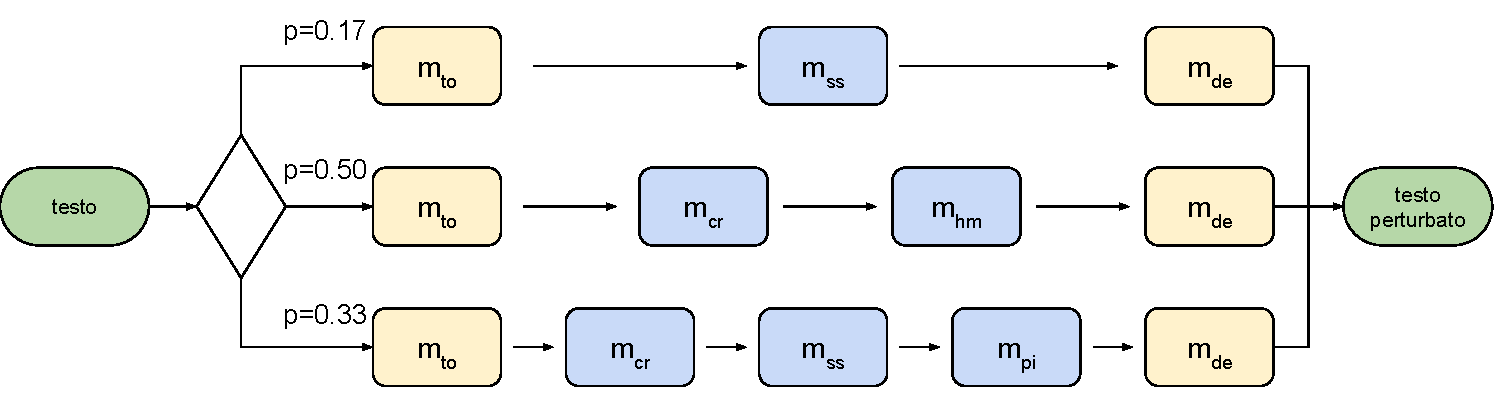
\includegraphics[width=\textwidth]{immagini/dataset/supex}
\caption{Schema della superpipeline descritta nell'esempio}
\label{fig:dst_supex}
\end{figure}



\section{Configurazione}
\label{dst:configurazione}
Nelle precedenti sezioni sono stati descritti la metodologia di creazione del dataset e il funzionamento del sistema di perturbazione. In questa sezione sono invece descritti i parametri usati per il sistema di perturbazione e quindi per la creazione del dataset.

\subsection{Pipeline e Superpipeline}
\label{sec:dst_pipsup}
In questa sottosezione sono definite le superpipeline usate per la perturbazione del dataset e le pipeline che le compongono. Sono state stabilite 3 tipologie di superpipeline, ognuna delle quali ha 3 livelli di intensità:

\begin{itemize}
\item \textbf{Token superpipeline}: sono superpipeline che introducono solo dei word error (\autoref{sec:met_introduzione}), ovvero errori contenuti all'interno di un singolo token che non impattano la tokenizzazione. Le token superpipeline sono identificate dai codici T1, T2, T3, dove T1 e T3 sono rispettivamente la superpipeline che introduce meno errori e quella che ne introduce di più.

\item \textbf{Segmentation superpipeline}: sono superpipeline che introducono solo dei word segmentation error (\autoref{sec:met_introduzione}), ovvero che dividono o uniscono uno o più token e che impattano quindi la tokenizzazione. Le segmentation superpipeline sono identificate dai codici S1, S2, S3, dove S1 e S3 sono rispettivamente la superpipeline che introduce meno errori e quella che ne introduce di più.

\item \textbf{Mixed Pipeline}: sono superpipeline che introducono sia word error che word segmentation error. Le segmentation superpipeline sono identificate dai codici M1, M2, M3, dove M1 e M3 sono rispettivamente la superpipeline che introduce meno errori e quella che ne introduce di più.
\end{itemize}

In totale sono definite 9 superpipeline (T1, T2, T3, S1, S2, S3, M1, M2, M3): questo numero permette di avere una buona granularità tenendo comunque contenuti i tempi durante la fase di testing.

\subsubsection{Pipeline}
Le superpipeline appena descritte sono formate dalla combinazione di più pipeline. Sono definiti tre tipi di pipeline:
\begin{itemize}
\item Token pipeline
\item Segmentation pipeline
\item Mixed pipeline
\end{itemize}
ognuna di queste tipologie di pipeline introduce gli stessi tipi di errore delle omonime superpipeline. Per ogni tipologia di pipeline sono definite 3 pipeline, ognuna della quali ha li stessi moduli con probabilità diverse.

\paragraph{Token pipeline} Una token pipeline è formata dai moduli presenti nella seguente \autoref{tab:dst_tkpip}:

\begin{table}[H]
\centering
\begin{tabular}{cccc}
\textbf{Posizione} & \textbf{Tipo Modulo} & \textbf{punct}\\ \hline
1	& \mto	& n.d 	\\
2	& \mcr	& n.d 	\\
3	& \mde	& n.d 	\\
\end{tabular}
\caption{Moduli presenti in una token pipeline}
\label{tab:dst_tkpip}
\end{table}

In \autoref{tab:dst_tkpipdef} sono definite le tre token pipeline. Nella tabella, $p_i$ indica la probabilità associata al modulo in posizione $i$.

\begin{table}[H]
\centering
\begin{tabular}{cccc}
\textbf{Codice} & \boldmath{$p_1$} & \boldmath{$p_2$} & \boldmath{$p_3$}  \\ \hline
$tok_1$	& n.d	& 0.1	& n.d 	\\
$tok_2$	& n.d	& 0.3	& n.d 	\\
$tok_3$	& n.d	& 0.3	& n.d 	\\
\end{tabular}
\caption{Definizione delle tre token pipeline}
\label{tab:dst_tkpipdef}
\end{table}



\paragraph{Segmentation pipeline}
Una segmentation pipeline è formata dai moduli presenti nella seguente \autoref{tab:dst_sgpip}:

\begin{table}[H]
\centering
\begin{tabular}{cccc}
\textbf{Posizione} & \textbf{Tipo Modulo} & \textbf{punct}\\ \hline
1	& \mto	& n.d 	\\

2	& \mhm	& n.d 	\\
3	& \mps	& , (virgola)	\\
4	& \mss	& n.d 	\\
5	& \mpi	& . (punto)	\\
6	& \mpi	& , (virgola)	\\
7	& \mpi	& ' (apostrofo) 	\\

8	& \mde	& n.d 	\\
\end{tabular}
\caption{Moduli presenti in una segmentation pipeline}
\label{tab:dst_sgpip}
\end{table}

In \autoref{tab:dst_sgpipdef} sono definite le tre segmentation pipeline. Nella tabella, $p_i$ indica la probabilità associata al modulo in posizione $i$.

\begin{table}[H]
\centering
\begin{tabular}{ccccccccc}
\textbf{Codice} 
& \boldmath{$p_1$} 
& \boldmath{$p_2$} 
& \boldmath{$p_3$}
& \boldmath{$p_4$}
& \boldmath{$p_5$}
& \boldmath{$p_6$}
& \boldmath{$p_7$}
& \boldmath{$p_8$}
\\ \hline
$seg_1$	& n.d	& 0.001	& 0.001	& 0.0025	& 0.005	& 0.005	& 0.005	& n.d\\
$seg_2$	& n.d	& 0.001	& 0.002	& 0.008		& 0.025	& 0.025	& 0.025	& n.d\\
$seg_3$	& n.d	& 0.01	& 0.02	& 0.05		& 0.1	& 0.1	& 0.1	& n.d\\
\end{tabular}
\caption{Definizione delle tre segmentation pipeline}
\label{tab:dst_sgpipdef}
\end{table}


\paragraph{Mixed pipeline} Le mixed pipeline derivano dalla composizione di una token pipeline con una segmentation pipeline. Le mixed pipeline sono definite in \autoref{tab:dst_mixpipdef}.

\begin{table}[H]
\centering
\begin{tabular}{cc}
\textbf{Codice} & \textbf{Definizione} \\ \hline
$mix_1$ & $seg_1 \circ tok_1$ \\
$mix_2$ & $seg_2 \circ tok_2$ \\
$mix_3$ & $seg_3 \circ tok_3$ \\
\end{tabular}
\caption{Definizione delle tre mixed pipeline}
\label{tab:dst_mixpipdef}
\end{table}


\subsubsection{Superpipeline}
Date le pipeline appena definite, le superpipeline si compongono come mostrato nella \autoref{tab:dst_suppipdefall}: ad ogni superpipeline sono associati i pesi di ciascuna delle sue pipeline.

\begin{table}[H]
\centering
\begin{tabular}{cccccccccc}
\textbf{Codice}
& \boldmath{$tok_1$} 
& \boldmath{$tok_2$} 
& \boldmath{$tok_3$} 
& \boldmath{$seg_1$} 
& \boldmath{$seg_2$} 
& \boldmath{$seg_3$} 
& \boldmath{$mix_1$}
& \boldmath{$mix_2$} 
& \boldmath{$mix_3$} 
\\ \hline
T1	& 6	& 4	& 1	& /	& /	& /	& /	& /	& / \\
T2	& 2	& 8	& 1	& /	& /	& /	& /	& /	& / \\
T3	& 1	& 6	& 4	& /	& /	& /	& /	& /	& / \\
S1	& /	& /	& /	& 6	& 4	& 1	& /	& /	& / \\
S2	& /	& /	& /	& 2	& 8	& 1	& /	& /	& / \\
S3	& /	& /	& /	& 1	& 6	& 4	& /	& /	& / \\
M1	& /	& /	& /	& /	& /	& /	& 6	& 4	& 1 \\
M2	& /	& /	& /	& /	& /	& /	& 2	& 8	& 1 \\
M3	& /	& /	& /	& /	& /	& /	& 1	& 6	& 4 \\
\end{tabular}
\caption{Definizione delle nove superpipeline}
\label{tab:dst_suppipdefall}
\end{table}



\subsection{Dataset}
In questa sottosezione sono descritte le istanze del dataset create e i loro parametri. Sono ricordati in seguito i parametri configurabili per la creazione di un dataset:
\begin{itemize}
\item $l_{min}$: lunghezza minima di una frase nel dataset.
\item $l_{max}$: lunghezza massima di una frase nel dataset.
\item \textit{Lingue}: lista di lingue consentite nelle frasi nel dataset.
\item \textit{Superpipeline}: lista di superpipelines usate per la perturbazione.
\item \textit{Dimensione}: numero di elementi che formano il dataset, se esso viene ridotto
\end{itemize}

In \autoref{tab:dst_dstconfig} sono elencate le versione del dataset definiti e i loro parametri:

\newcommand{\dsta}{dst@50}
\newcommand{\dstb}{dst@100}

\begin{table}[H]
\centering
\begin{tabular}{cccccc}
\textbf{Codice} & \boldmath{$l_{min}$} & \boldmath{$l_{max}$} & \textbf{Lingue} & \textbf{Superpipeline} & \textbf{Dimensione}\\ \hline
\dsta & 8 & 50 & [it] & \tiny[T1, T2, T3, S1, S2, S3, M1, M2, M3]& 10000\\
\dstb & 20 & 100 & [it] & \tiny[T1, T2, T3, S1, S2, S3, M1, M2, M3]& 10000\\
\end{tabular}
\caption{Configurazione delle versioni del dataset}
\label{tab:dst_dstconfig}
\end{table}

Le due versioni del dataset differiscono solamente nella lunghezza massima e minima delle frasi. In questo modo sarà possibile testare quanto la lunghezza di una frase (e quindi il contesto intorno ad un errore) influisca sulle performance di correzione. Questi aspetti, insieme ai risultati dei testi, sono approfonditi nel \autoref{sec:test}.






